\subsubsection{InSynth proof trees}

InSynth proof trees are the output of the resolution phase and represent ``proofs'' of expressions construction, in the sense that expressions of the required type can indeed by constructed out of leafs as declarations from the given program environment.
With respect to the encoding (described in \ref{subsubsec:encoding_the_environment}), such proofs only bear information that valid expressions can be constructed with combining some specific ground types together with nested sub-expressions.
Such combination is derived by using the rule presented in Figure \ref{fig:appabs_rule} and uses simplified ground type reasoning - therefore it does not directly encode how should the synthesized code snippets actually look like when given as suggestions to the developer.
InSynth proof trees include the information about correspondence between used ground types and program declarations in order to allow syntactically synthesis of valid code snippets.
In addition to including information about program declarations, since the resolution is driven by weights of such declarations, proof trees also include information about the weights of encoded ground types.

An example that depicts the outline of the structure of InSynth proof trees which are inputs to the code generation phase is depicted in Figure \ref{fig:InSynth_tree_example}.

\begin{figure}[ht]
\centering
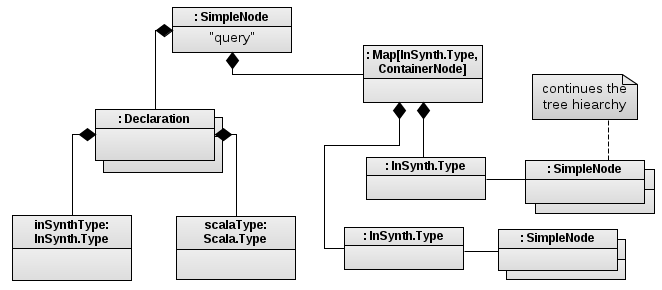
\includegraphics[width=0.45\textwidth]{proof_tree}
\caption{Object diagram with an InSynth proof tree example}
\label{fig:InSynth_tree_example}
\end{figure}

% The general idea behind such structure of nodes (and thus the tree) is to allow
% generating expressions (of the target code) which have the required type by
% using given declarations and combining them with terms that are generated by
% considering immediate sub-trees.

The proof tree consists of nodes (implemented as \textit{SimpleNode} classes) that carry the information about which ground types (given by \textit{Declaration} class) can be combined with expressions of types defined by the parameters map.
The parameters map represents information on how to construct sub-expressions of a given node and maps a type (\textit{InSynth.Type}) to a set of subtrees (contained in the \textit{ContainerNode} object).
Each \textit{Declaration} consists of the simplified ground type \textit{InSynth.Type} which can be used in the combination its corresponding program declaration \textit{Scala.Type} which stores the language-specific information that are needed for the actual code generation. 

Note that according to the resolution phase (which uses the \textsc{AppAbs} rule) and simplified representation of \textit{ground types}, each node in the proof tree provides information how to synthesize expression of the ``rightmost'' primitive type, $T_1$ in the rule, while having variables of types in $S_1$ added to the typing context (e.g. for synthesis of Scala type \textit{Int =\textgreater Char =\textgreater String} the proof tree would provide information on synthesis of expressions of type \textit{String} while having variables of types \textit{Int, Char} added to the typing context).

% For a node $n$ (of type $SimpleNode$), in order to generate expressions of type
% $n.goalType$ one must either use some declaration $d$ from
% $n.declarations$ which matches the $goalType$ directly (e.g. when $goalType = d.type = Int$ and
% $d$ refers to a field declaration of type $Int$) or apply needed arguments to
% $d$ if $d.type$ is a function type, which returns $goalType$ (e.g. when
% $goalType = Int$ and $d.type = (Char => Int)$, the process must get expressions of type
% $Char$ in order to apply them to $d$).
% One special case can happen if the goal type is a function type $X=>Y$ and in
% that case a function which takes parameters described by $X$ and which
% returns a term of type $Y$ can be generated.
% Terms of type $Y$ can be synthesized by taking also those parameters into
% consideration - $LeafNode$ indicates that the term(s) should be looked up in
% the current typing context.

\subsubsection{Weighted search}

Weighted search is the first step in the code generation process and its main goal is to extract only the needed number $N$ of the most optimal combinations in terms of associated weights.
The result of this step is a proof tree that contains only a subset of nodes from the original, input proof tree such that the belonging nodes are sufficient in constructing (at least) $N$ code snippets with the lowest weight that need to be suggested to the developer\footnote{more specifically the output of this step uses a slight variation of the proof tree representation and due to the nature of the simplified representation, is guaranteed to hold information to generate $N$ or more code snippets}.  
The rationale behind this step is that the resolution step may, due to combinatorial explosion, output complex proof trees with a large number of nodes and the code generation phase can benefit from its pruning to achieve better responsiveness of the typing assist.
After this step, the unnecessary nodes are removed from the proof tree and the output entails only the necessary information for construction of most optimal solutions based on the assigned weights of program declarations.

The algorithm that accomplishes the weighted search is based on the uniform-cost search which is a search algorithm used for traversing weighted tree structures \cite{russel2003ai}.
The search begins at the root node and continues by visiting the next node which has the least total cost from the root.
Nodes are visited in this manner until a goal state is reached.


The main difference is that in our case there is no single global goal state.
When a subtree is fully explored its cumulative weight serves as a weighted goal for constructing an expression corresponding to that subtree.
When the root of the tree is fully explored we are sure that at least one expression can be combined in order to synthesize the goal (query) type.
Number of expressions a subtree can combine is equal to the product of number of possible declarations and each of its explored parameter subtrees.

The weighted search algorithm is depicted in Algorithm \ref{alg:weighted_search}.

\begin{algorithm}[ht]
\caption{Weighted search}
\label{alg:weighted_search}
\begin{algorithmic}[1]

\REQUIRE{root node $r$}

\STATE{enqueue $r$}

\WHILE{queue is not empty}
\STATE dequeue node $n$
\IF{$n$ is not pruned} 
\STATE update weights of nodes up the tree and prune nodes according to their updated weights if needed
\IF{$n$ is a leaf node}
\STATE mark the subtree as explored and propagate to $r$
\IF{number of combinations at $r$ is $\geq N$}
\STATE enable pruning of nodes
\ENDIF
\ENDIF
\FORALL{children $c$ of $n$}
\IF{$c$ is not visited}
\STATE enqueue $c$
\ENDIF
\ENDFOR
\ENDIF
\ENDWHILE
\RETURN $r$
\end{algorithmic}
\end{algorithm}

The algorithm gradually explored nodes according to their weights (set of visited nodes is maintained since in general there can be cycles in the proof tree), prunes the subtrees that ought to construct expressions of larger weight and finishes when the resulting tree contains nodes for construction of at least $N$ expressions.
Note that the algorithm does not stop until it exhausts the priority queue of unexplored nodes and only examines nodes that can explore optimal subtrees (with total weight less than previously explored subtrees).

The design of the algorithm allows implementation of incremental updates of proof trees from the resolution phase (which would add unexplored nodes to the priority queue) and it allows its implementation to support some more sophisticated policies for nodes weight calculation (instead of summing the weights of subtree node it can search for package declarations path matches, specific subtree pattern matches, etc.). 

\subsubsection{Intermediate transformation}

In the second step of the code generation phase, an intermediate transform is performed on the input (pruned) proof tree.

\begin{figure}[ht]
\centering
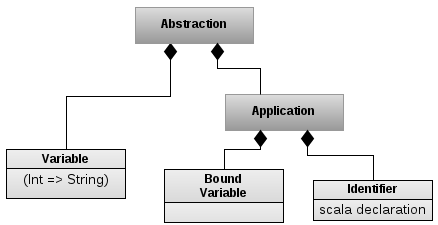
\includegraphics[width=0.35\textwidth]{intermediate_example}
\caption{Intermediate representation tree example}
\label{fig:intermediate_example}
\end{figure}

The goal of this step is to produce intermediate representation trees which combine program declarations and combinations encoded in proof trees and contain enough information about the structure of the code to be synthesized.
The resulting trees in the intermediate representation are very similar to terms from the \LC and thus precisely encode information about abstractions and applications to be used in the synthesized code.\footnote{In spite of containing more precise information about the code to be synthesized, the intermediate representation offers an abstract way of encoding the code structure so that potentially other programming languages can be supported for code snippet generation}

An example of a tree in intermediate representation is given in Figure \ref{fig:intermediate_example}.
The example encodes a single expression in which an identifier from the program context is applied to the function term declared in the top abstraction.
The intermediate representation trees contain abstraction nodes which correspond to abstraction terms in the \LC but which can bind multiple terms (in order to correspond syntactically more powerful abstraction counterparts in Scala), application nodes which represent an application in the \LC (again, the distinction is that they can include multiple parameters), identifier nodes that represent program declarations and bound variables that represent usage of terms declared by some abstraction at higher levels in the tree.
Important property of the intermediate representation is that each node in the place of its sub-terms can contain multiple nodes (a set of nodes) in order to allow encoding that multiple expressions of the same type can be used whenever an expression of that type is required.

We will now describe the algorithm for transforming InSynth proof trees to intermediate representation trees. 

\begin{algorithm}[ht]
\caption{Transformation procedure}
\label{alg:transformation}
\begin{algorithmic}[1]

\REQUIRE{InSynth proof tree rooted at $r$}

\STATE \COMMENT{$r$ is the query node which has type $(T \rightarrow \bot)$}

\RETURN{Transform($\emptyset$, $r$, $\bot$)}

\end{algorithmic}
\end{algorithm}
The entry point to the transformation is depicted in Algorithm \ref{alg:transformation}.
Its input is the (pruned) proof tree, more specifically its root $r$ which contains the initial \textit{query type} $T \rightarrow \bot$, where $T$ is the type of expressions we want to synthesize.
The algorithm initializes an empty typing context and calls the recursive \textit{Transform} procedure given in Algorithm \ref{alg:transform_call} on the root node with an empty context and with $\bot$ as the goal type.
Note that if an expression of type $\bot$ is derived then its immediate sub-expressions will be of the required type $T$.


%\floatname{algorithm}{Procedure}
%\renewcommand{\algorithmicrequire}{\textbf{Input:}}
%\renewcommand{\algorithmicensure}{\textbf{Output:}}
%\renewcommand{\algorithmicreturn}{\textbf{add to solution set}}

\begin{algorithm}[ht]
\caption{Transform}
\label{alg:transform_call}
\begin{algorithmic}[1]

\REQUIRE{context $\Gamma$, current node $n$, goal type $t$}
% \COMMENT{The procedure requires:}
% \STATE\COMMENT{since the call is recursive, the term resolved in this
% procedure $x$, will be applied to $t$, i.e. we will have $\lambda$ expression $(t x)$}
\STATE\COMMENT{context $\Gamma$ is the current typing context}

\IF{$t$ is of the form $(X \Rightarrow Y)$}
\FORALL{type $X_i$ in $X$ according to real type}
\STATE{let be fresh variable $x_i$ of type $X_i$}
\ENDFOR
\STATE{let $a$ be an abstraction that bounds all variables in $X$}
\COMMENT{$a = (\lambda x_1:X_1. (\lambda x_2:X_2. \ldots (\lambda
x_n:X_n.\textrm{ ``\_``})))$}
\FORALL {$t'$ in Transform declarations($\Gamma \cup (\bigcup_i x_i:X_i)$, $n$, $Y$)}
\RETURN {$a$ [$\textrm{ ``\_``}\rightarrow t'$]}
\STATE\COMMENT {plug $t'$ into the abstraction $a$ in place of ``\_``}
\ENDFOR
\ELSE
\RETURN Transform declarations($\Gamma$, $n$, $t$)
\ENDIF

\end{algorithmic}
\end{algorithm}
The recursive Transform, depicted in Algorithm \ref{alg:transform_call} expects as inputs the current node $n$ in the proof tree, current typing context $\Gamma$ and a goal type $t$, to which expressions constructed from subtree $n$ should typecheck to.

It checks the form of $t$ (at the first call, $t$ is equal to the \textit{query type}):
\begin{itemize}
  \item if $t$ is not a function type - according to the rule \textsc{AppAbs} by which the resolution step is derived, $t$ represents $T_1$ and $S1= \{\}$ - the transformation proceeds immediately recursively to get sub-expressions of type $T_1$
  \item if $t$ is a function type $X \rightarrow Y$ - according to the rule \textsc{AppAbs}, $t$ represents $S_1 \rightarrow T_1$ - an abstraction terms(s) are formed in order to introduce variables of types found in $X$ and the transformation proceeds recursively to get sub-expressions of type $T_1$ under the updated context
\end{itemize}
The transformation of type $T_1$ in both cases is achieved with a helper procedure given in Algorithm \ref{alg:make_declarations}, which scans the available declarations in the current node and current context in order to transform sub-expressions.


\begin{algorithm}[ht]
\caption{Transform declarations}
\label{alg:make_declarations}
\begin{algorithmic}[1]

\REQUIRE{context $\Gamma$, current node $n$, goal type $t$}
\STATE {search for declarations that can return $Y$ type in declarations contained in the node $n$ and in $\Gamma$}
\STATE {denote the result set of declarations as $D$}
\FORALL {declarations $d$ from $D$}
\IF {$d$ has no parameters}
\RETURN {identifier or bound variable node for $d$}
\ELSE
\FORALL {parameters $p_i$ of type $t_i$ in $d$}
\FORALL {child nodes $n'$ that are contained in container node $parameters(t_i)$}
\STATE {let $S_i$ be the result of Transform($\Gamma$, $n'$, $Y$)}
\COMMENT{set of nodes that represent sub-expressions of type $t_p$}
\ENDFOR
\ENDFOR
\RETURN {application node ($d$ $S_1$ $S_2$ \ldots $S_n$)} \COMMENT{if $d$ has $n$ parameters}
\ENDIF
\ENDFOR

\end{algorithmic}
\end{algorithm}
The \textit{Transform declarations} procedure scans declarations at the given node and the context to find suitable declarations that can transform to a given goal type.
Such declarations may be returned directly as identifier or bound variable nodes (do not require application to them) or as applications of recursively transformed parameters of appropriate type.
Note that intermediate representation allows set of nodes to be included for each application and abstraction nodes thus enables representing multiple expressions with one tree.

% \textit{Note:} The line $return$ $x$ in the procedure $Transform$ does not
% designate a conventional return call from a function, but rather an indication that such
% result $x$ should be returned as one of the results (more
% specifically, $Transform$ returns a set of terms which contains all terms which
% are prepended with the $return$ command in the Algorithm \ref{alg:transform_call}).

\subsubsection{Code snippet generation}

The code snippet generation represents the final step in the code generation phase and it takes intermediate representation as input and produces code snippets in a target language, namely Scala, and ranks them according to their weight.

This step is based on a tree traversal transformation algorithm which traverses the intermediate representation tree and produces a set of code snippets.
Since the intermediate representation tree encodes the program structure and also allows multiple sub-trees in its abstraction and application nodes, the code snippet generation step has to consider and collect every possible expression that is included in the intermediate representation tree (and returns only the specified number of them, ranking them by weight).

Although the intermediate representation precisely encodes the structure of code snippets to be generated in terms of \LC terms, the code snippet generation step has to consult the information provided by the program declarations in order to be able to generate syntactically correct code and also to be able to simplify the resulting code as much as possible.
These language-specific transformations include usage of correct syntactical constructs (e.g. if the application represents a construction of an object, keyword \textit{new} has to be outputed), usage of syntactic sugar instances (e.g. omitting dot, parentheses and \textit{apply} in certain method calls) and general simplification steps (e.g. omitting of explicitly given types to expressions).

Resulting code snippets are encoded as a set of Scala pretty print documents (\textit{Scala.text.Document} objects) which are then transformed by custom-indentation defined properties to strings and reported back to the IDE (the output of such objects can be then processed with Scala format and refactoring libraries in order to have visually better suggestions reported to the developer, as described in architecture section in \cite{scala_dev}).
